\chapter{Introduction}

\section{Quantum Chromodynamics}
Relativistic deep-inelastic collisions of large ions produce high-energy interactions that allow for studies of High Energy Density (HED) matter. HED matter studied at ALICE from p-p, Pb-Pb, and Xe-Xe collisions is a mess of standard model particles called the Quark-Gluon Plasma (QGP). QGP is a medium of strongly-interacting particles that can reach temperatures higher than $10^{12}$ Kelvin, where the energy density is so high that interactions produce quarks that are asymptotically free. This is in the perturbative domain of quantum chromodynamics (QCD) because quarks and gluons are separated by short distances and have large exchanges of momentum, reducing the effect of gluonic self-interactions.
As the QGP expands, the energy density reduces and asymptotic freedom is no longer an appropriate approximation. Hadrons in the QGP interact to form baryons and mesons during cooling, a process referred to as rehadronization. The newly formed quark matter expands and produces jets that lose energy as they interact with the QGP. The energy loss of the jets as they traverse the QGP is known as jet quenching, and studying this process is critical to understanding the gaps between perturbative and lattice QCD \cite{QCD_Review}. Heavy ion collision experiments are at the frontier of the high-energy region of the phase space for QGP. Fig. \ref{fig:QGP_Phase_Diagram}, from \cite{QCDPhaseDiagram}, shows the phase diagram for QGP in terms of the Baryochemical Potential $\mu_B$ and the Temperature. 


\begin{figure}
    \centering
    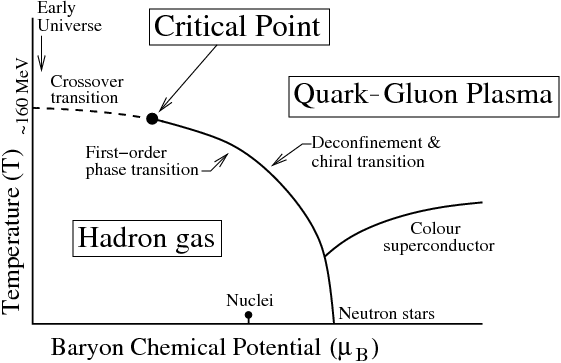
\includegraphics[width=0.6\textwidth]{figures/ALICE/QGP_Phase_Diagram.png}
    \caption{Phase diagram for the Quark-Gluon Plasma. Accelerator experiments with heavy ions allow for the exploration of the phase transitions between Hadron Gas and QGP. 1 MeV$\sim 10^{10}$K 
    \cite{QCDPhaseDiagram}}
    \label{fig:QGP_Phase_Diagram}
\end{figure}


\section{CERN Large Hadron Collider}
\begin{figure}[H]
    \centering
    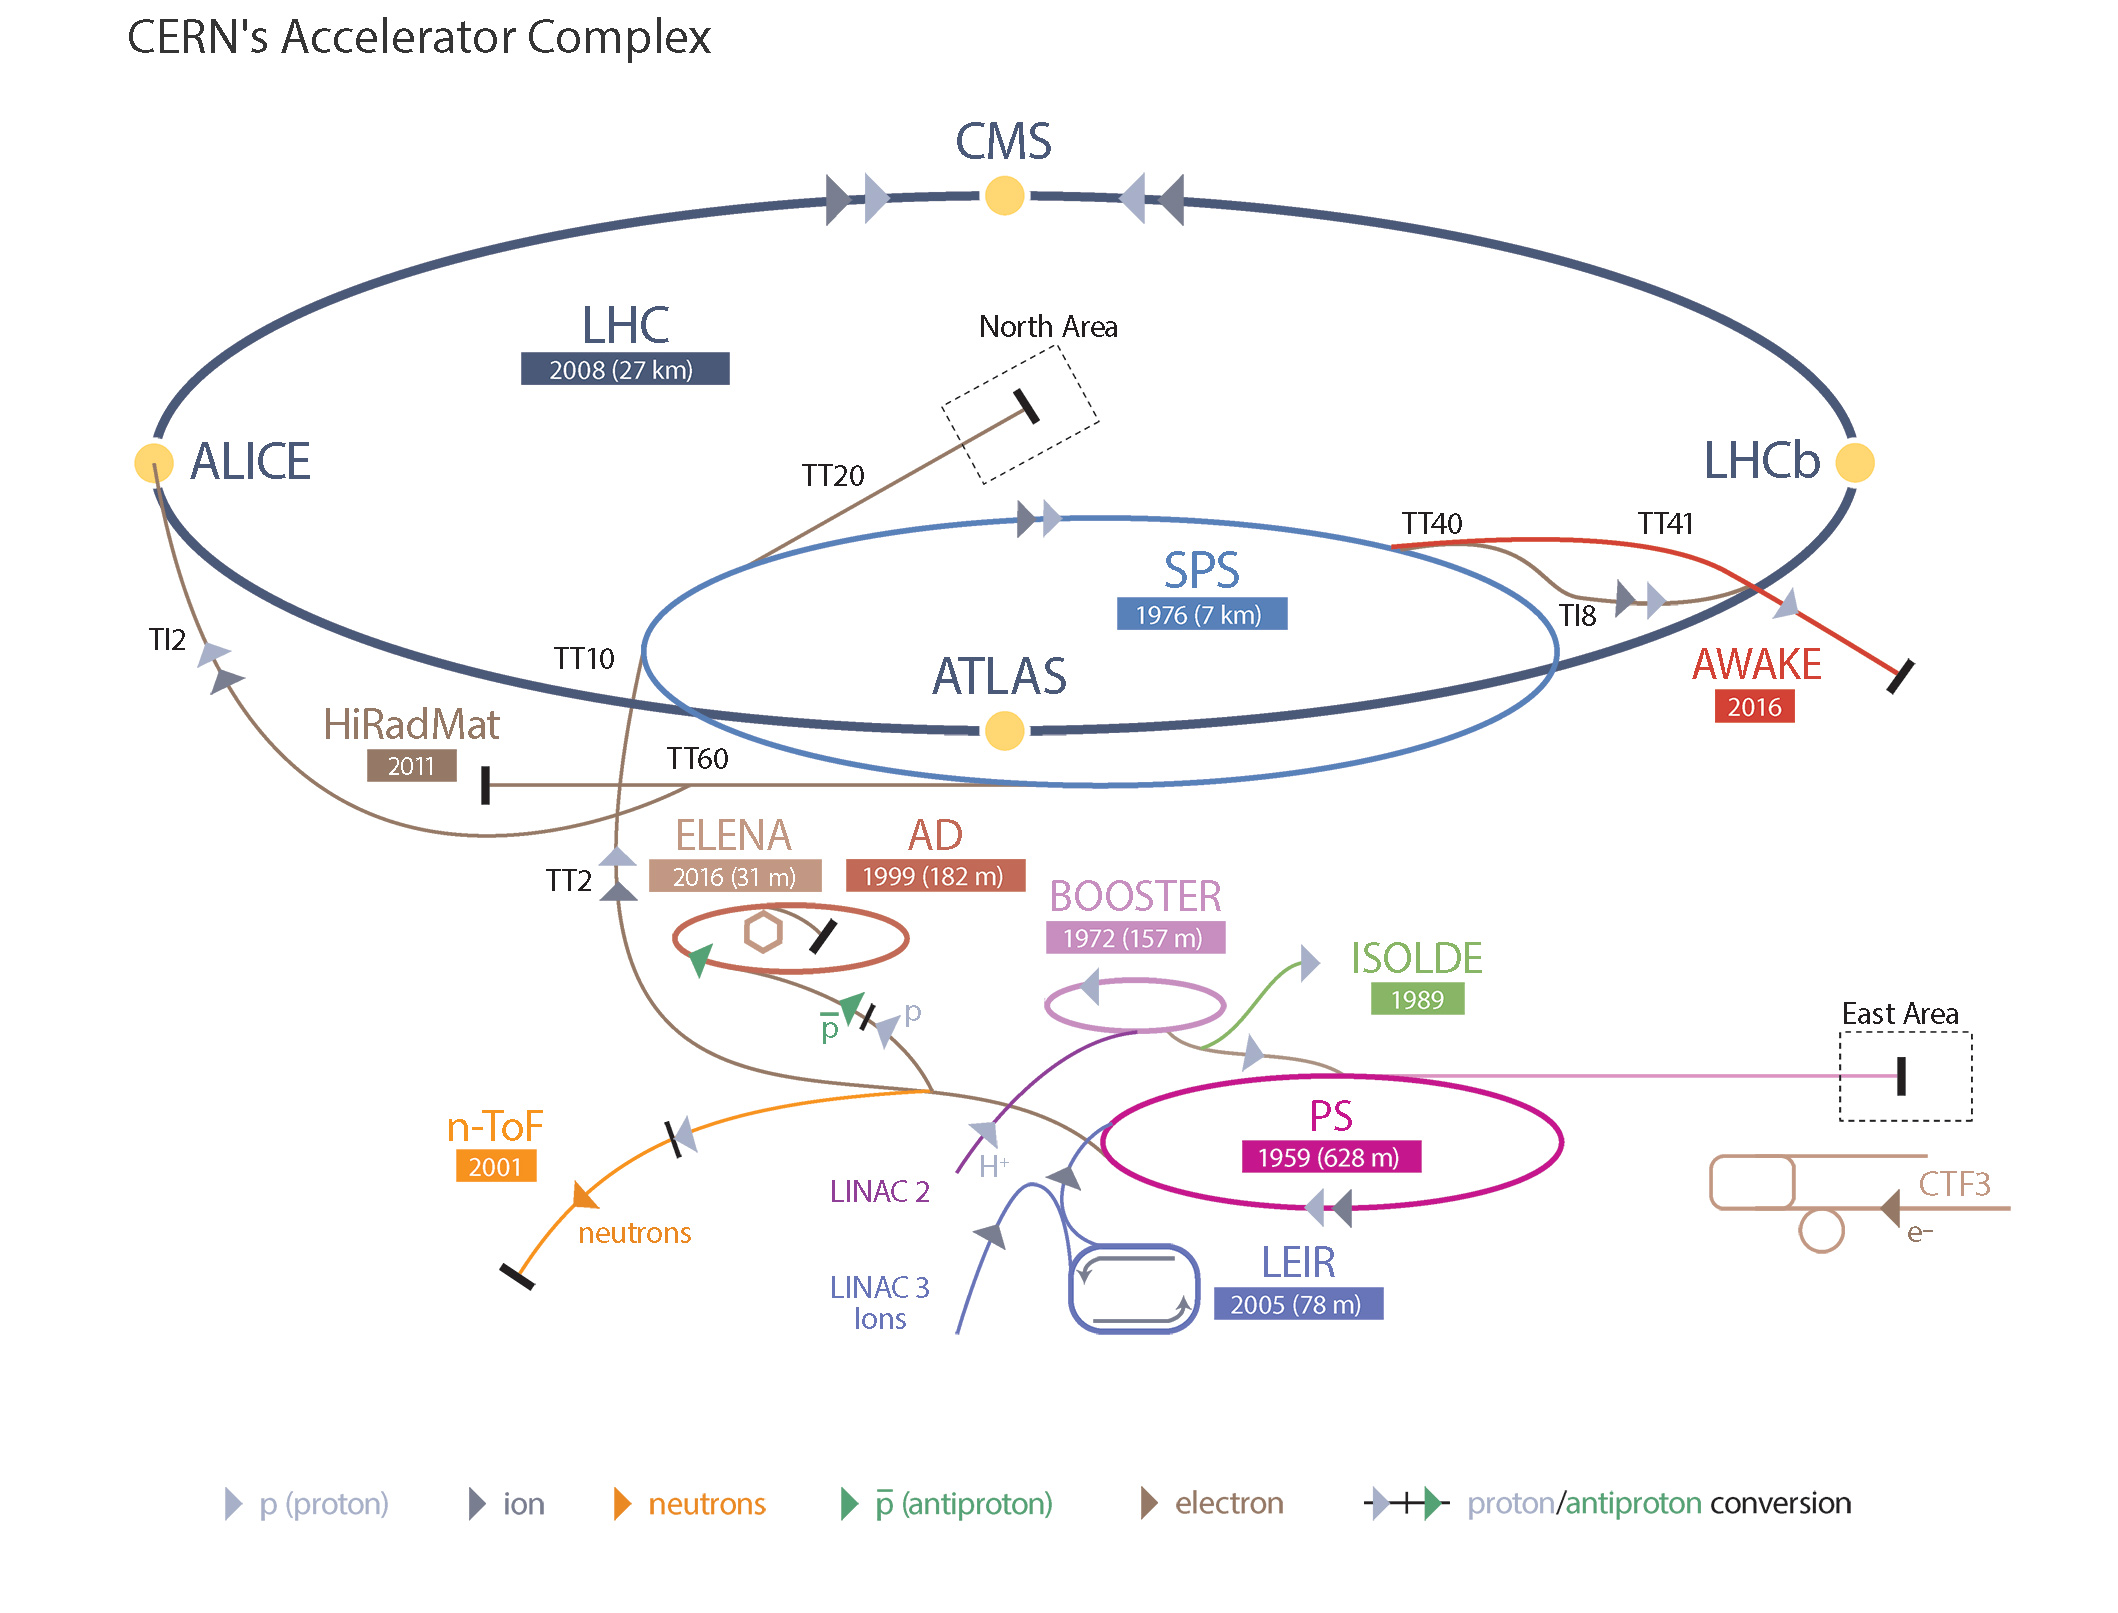
\includegraphics[width=0.7\textwidth]{figures/CERN/LHC_accelerator_complex.jpg}
    \caption{Accelerator complex at CERN Large Hadron Collider \cite{CernAcceleratorComplex}}
    \label{fig:CERN_Accelerator_Complex}
\end{figure}

The European Council for Nuclear Research (CERN) is one of the largest scientific organizations in the world, where scientists are engaged in the study of the fundamental constituents of the universe. This exploration of the smallest length and time scales is done using the most advanced technology available. CERN's Large Hadron Collider hosts a collection of accelerator-based experiments that study the way particles interact at very high energies, which gives us clues about the fundamental laws of physics. 

The Large Hadron Collider (LHC) is a 27 km ring of superconducting magnets and accelerating cavities first turned on in September 2008. Particle bunches are accelerated in opposite directions and countercirculate around the ring at energies of up to 7 TeV, guided by magnets cooled to near 1 Kelvin using liquid helium, far colder than space. The particles are then directed to one of four main experiments on the LHC: ALICE, ATLAS, CMS, and LHCb. Each experiment has a detector-based tracking system that measures information about collisions such as the energy, position, transverse momentum of produced particles, and the centrality and multiplicity of collision events. The LHC accelerator complex is shown in Fig. \ref{fig:CERN_Accelerator_Complex}.

CERN uses the data collected by these experiments to search for new interactions and particles like the Higgs boson, discovered in 2012 \cite{Higgs}. The data throughput of the LHC is huge; thousands of scientists spend months to years analyzing the data produced by the experiments at the LHC, often to reduce the parameter space of a proposed interaction mode, or to discover and test completely new physics.

Currently, the LHC is in its second Long Shutdown (LS2), where scientists upgrade and replace many of the accelerator and detector components. LHC Run 3 will begin in 2021 and continue until 2025. The long term schedule for the LHC is shown in Fig. \ref{fig:CERN_Timelne}.
\begin{figure}[H]
    \centering
    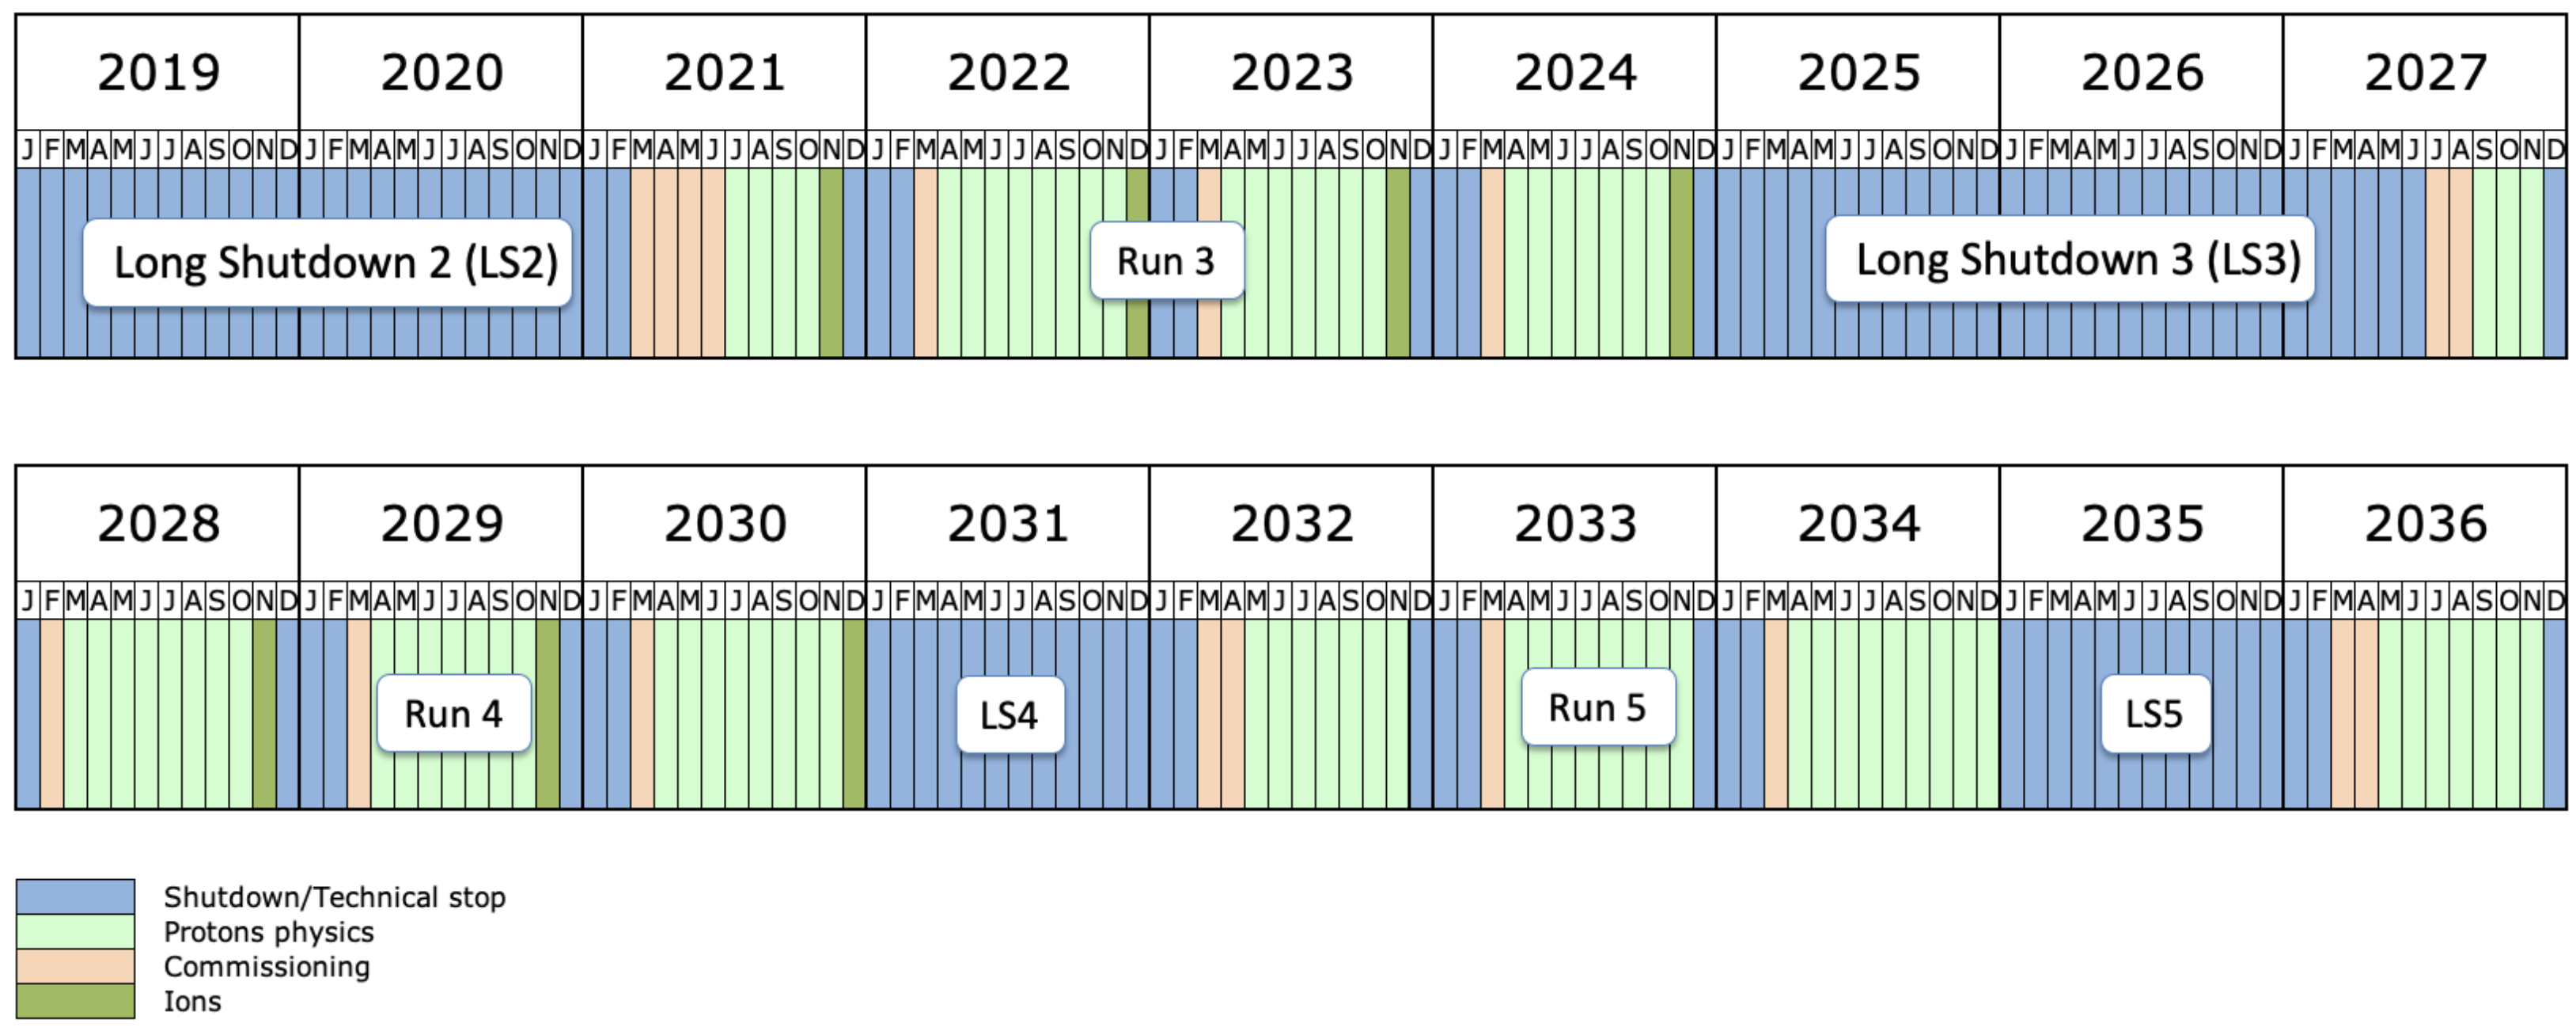
\includegraphics[width=\textwidth]{figures/CERN/LHC_Timeline.png}
    \caption{Long term schedule for LHC from 2019 through 2036 \cite{CernLongTermSchedule}.}
    \label{fig:CERN_Timelne}
\end{figure}

\section{A Large Ion Collider Experiment}

\begin{figure}[H]
    \centering
    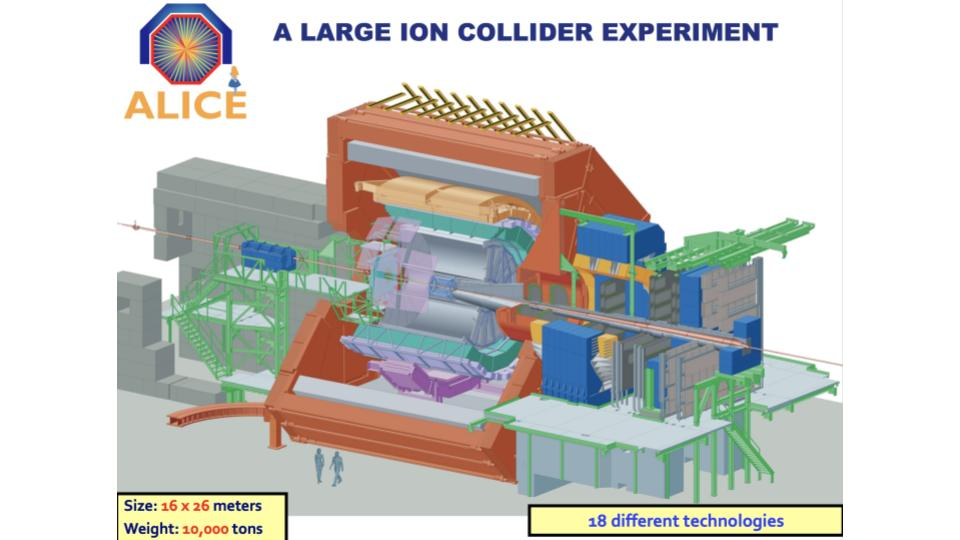
\includegraphics[width=0.6\textwidth]{figures/ALICE/alice_detector.jpg}
    \caption{Schematic cross-sectional view of the ALICE detector system \cite{ALICE_Schematic}}
    \label{fig:ALICE_DETECTOR}
\end{figure}

ALICE is one of the four main experiments at the LHC. A diagram of the upgraded ALICE detector is shown in Figure \ref{fig:ALICE_DETECTOR}\cite{ALICE_Schematic}. ALICE studies the QGP and strong interactions by detecting and tracking partons, measuring centrality, multiplicity, and energy of collisions. Tracking jets and rehadronization processes as they occur in the detector is incredibly difficult, but we observe the outcome of these processes using a variety of detectors including gaseous drift chambers, Cherenkov photomultipliers, scintillators, pixel trackers, and calorimeters. ALICE sites inside the L3 solenoidal magnet, the largest normal-conducting magnet in the world, with modest uniform 0.25 T field over the full central detector barrel.  This experiment is at the intersection of advanced technologies and impressive engineering feats. 


\section{ALICE Fast Interaction Trigger}
Hardware triggers based on event multiplicity, transverse momentum, and calorimeter energy provide
event selectivity that allows sampling of the full luminosity of particle beams that collide at ALICE. To study the QGP, event selection requires a minimum bias trigger. In ALICE, the detector that will provide this trigger for Run 3 and beyond, is called FIT, the Fast Interaction Trigger detector. FIT is a system of detectors that measure the key parameters to determine whether a signal that we pick up is worth tracking; if the appropriate combination of multiplicity, energy, location, time, and transverse momentum are measured, FIT sends a signal to other detectors in ALICE to begin data acquisition (DAQ). Fig. \ref{fig:FIT_IN_ALICE} shows two of the subdetectors within FIT as they are positioned in ALICE \cite{FIT_IN_ALICE}. 

\begin{figure}[H]
    \centering
    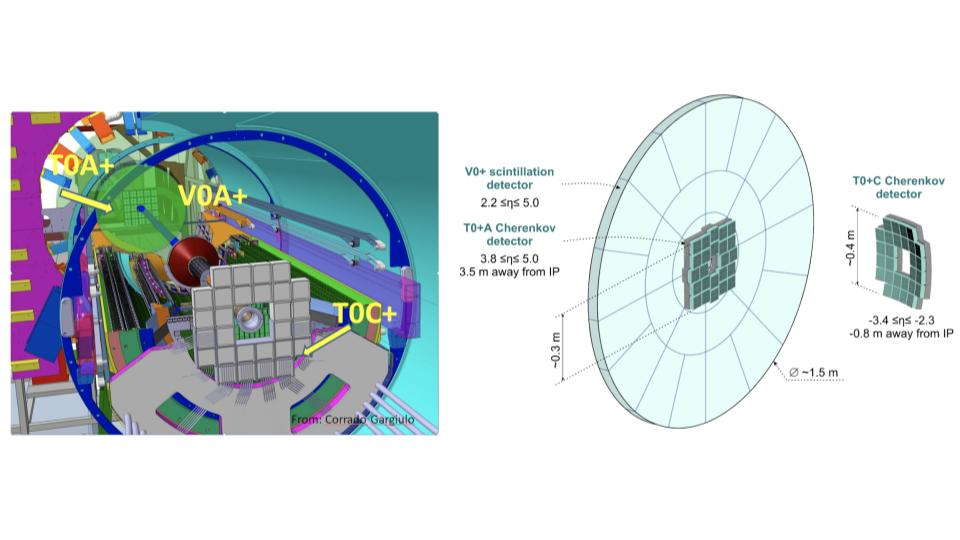
\includegraphics[width=0.8\textwidth]{figures/ALICE/FIT_in_ALICE.jpg}
    \caption{Fast Interaction Trigger positioned inside ALICE, shown in perspective view (left) and in component view (right) \cite{FIT_IN_ALICE}}
    \label{fig:FIT_IN_ALICE}
\end{figure}

\section{Online-Offline Computing System}

During LHC Run 3, ALICE is expecting an integrated luminosity of 13 ${nb}^{-1}$ of Pb-Pb collisions in minimum bias mode, with an interaction rate of approximately 50 kHz. To capture maximal information, some detector systems are being upgraded for continuous readout to prevent trigger deadtime losses due to event pileup. This increases the data throughput of ALICE up to the order of TB/s, corresponding to a data volume two orders of magnitude greater than Run 1. ALICE has introduced a new computing framework, $O^2$, which is composed of optimized software and large computing facilities that are designed specifically for detection and analysis of physics events \cite{O2_TDR}.

Continuous readout of some detectors is a drastic difference from previous techniques. Data collection is achieved with many constant data streams to the computing system. Data flows will be separated into Time Frames, regular intervals synchronized with the LHC clock. Because the data are local and independent the triggering process can be performed with parallel computing. This allows for the simultaneous DAQ and processing, which is very useful for data volume reduction. Results are stored in Tier 0 of the CERN data center or in the $O^2$ farm. These results are further processed later using resources from the CERN Computing Grid and are available for analysis to anyone with access to the Grid. Fig \ref{fig:O2_Schematic} shows the flow of data from detector to the grid, along with the iterated compression and reconstruction of data. 


\begin{figure}[H]
    \centering
    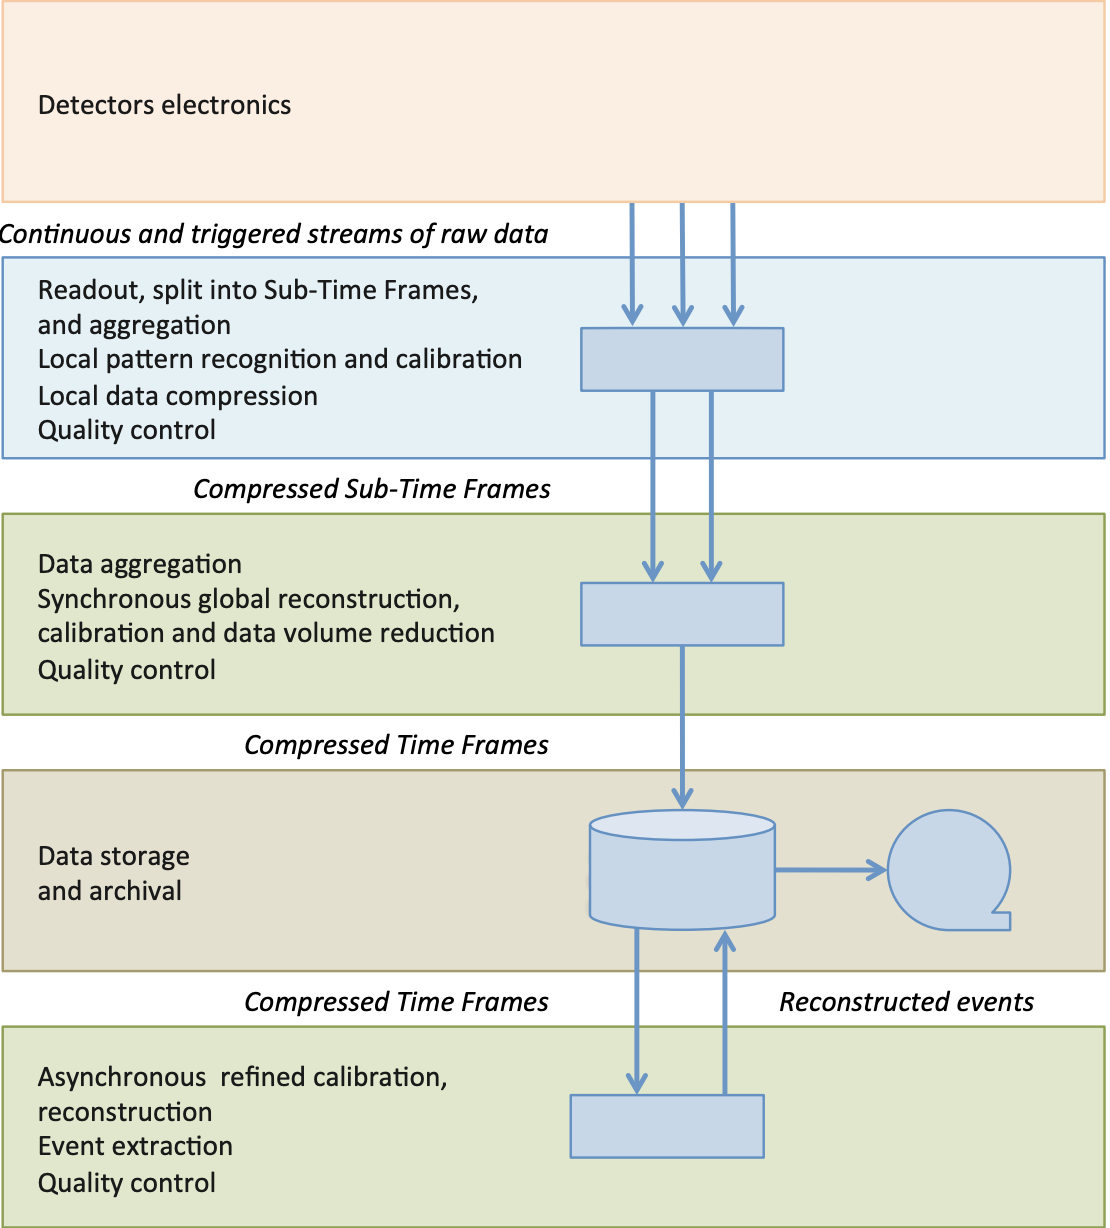
\includegraphics[width=0.6\textwidth]{figures/O2/O2_schematic.png}
    \caption{Diagram of the data flow from the ALICE detectors through the $O^2$ computing system. Compression and reconstruction are iterated until both data size and quality are optimized \cite{O2_TDR}}
    \label{fig:O2_Schematic}
\end{figure}

